% =====================================================================
%  I CONAEX - Resumo expandido
%  Identificação de padrões de dificuldade em leitura e escrita via XAI
%
%  Overleaf: Menu > Compiler: pdfLaTeX | Main document: main.tex
%
%  Formatação do modelo oficial do evento: Times 12, espaçamento simples,
%  margens superior e esquerda de 3 cm e inferior e direita de 2 cm, texto
%  justificado, recuo de 1,25 cm, logo só na 1a página, linha em branco
%  entre as seções, citações (NBR 10520:2023) e referências (NBR 6023) ABNT.
%
%  VERSÃO COM OU SEM IDENTIFICAÇÃO
%  O edital pede dois PDFs. Para a versão SEM identificação, troque
%  \identificacaotrue por \identificacaofalse logo abaixo e compile de novo.
%  Isso tira o nome dos autores e o link do repositório.
% =====================================================================
\documentclass[12pt,a4paper]{article}

\newif\ifidentificacao
\identificacaotrue      % \identificacaofalse para a versão sem identificação

% ---------------------------------------------------------------- idioma e fonte
\usepackage[T1]{fontenc}
\usepackage[utf8]{inputenc}
\usepackage[brazilian]{babel}
\usepackage{mathptmx}             % Times
\usepackage{icomma}                % vírgula decimal em modo matemático
\usepackage{microtype}

% ---------------------------------------------------------------- página
\usepackage[a4paper,top=3cm,left=3cm,bottom=2cm,right=2cm]{geometry}
\usepackage{indentfirst}
\setlength{\parindent}{1.25cm}
\setlength{\parskip}{0pt}
\pagestyle{empty}
\frenchspacing

% ---------------------------------------------------------------- seções
% Negrito, caixa alta, tamanho 12, com uma linha em branco antes e depois.
\usepackage{titlesec}
\titleformat{\section}{\normalfont\normalsize\bfseries}{\thesection}{0.5em}{}
\titlespacing*{\section}{0pt}{\baselineskip}{\baselineskip}
\titleformat{\subsection}{\normalfont\normalsize\bfseries}{\thesubsection}{0.5em}{}
\titlespacing*{\subsection}{0pt}{0.5\baselineskip}{0pt}

% ---------------------------------------------------------------- tabelas e figuras
\usepackage{graphicx}
\usepackage{booktabs}
\usepackage{array}
\usepackage{xcolor}
\usepackage{caption}
\captionsetup{labelsep=endash,font=normalsize,labelfont=normalsize,
              justification=centering,singlelinecheck=false}
\captionsetup[table]{position=above,skip=4pt}
\captionsetup[figure]{position=below,skip=6pt}
\newcommand{\fonte}[1]{\par\vspace{2pt}{\small Fonte: #1}}

% ---------------------------------------------------------------- citações ABNT
% Autor-data, como no modelo: (Rudin, 2019); (Dias et al., 2023).
\usepackage{natbib}
\bibpunct{(}{)}{;}{a}{,}{,}
\renewcommand{\bibsection}{\section*{REFERÊNCIAS}}
\setlength{\bibhang}{0pt}
\setlength{\bibsep}{\baselineskip}
\renewcommand{\bibfont}{\raggedright}

\usepackage{xurl}
\urlstyle{same}
\usepackage[hidelinks]{hyperref}

\newcommand{\Rdois}{$R^2$}

\begin{document}

% =====================================================================
\begin{center}

\includegraphics[width=6.77cm]{figuras/logo_conaex.png}

\vspace{\baselineskip}
\textbf{IDENTIFICAÇÃO DE PADRÕES DE DIFICULDADE EM\\ LEITURA E ESCRITA VIA XAI}

\ifidentificacao
\vspace{\baselineskip}
% Orientador por último, como pede o edital.
ALLYSSON SOUZA; DÉBORA ZANOELLO; MARCELO CARVALHO REZENDE FARIA; ANDERSON ARA
\fi

\vspace{\baselineskip}
\textbf{RESUMO}
\end{center}

\noindent
Um assistente proativo de leitura e escrita precisa de duas previsões: o ritmo
habitual de digitação de uma pessoa, referência para reconhecer quando ela
hesita, e os termos de um texto que ela tende a achar difíceis. O objetivo deste
trabalho foi verificar se modelos interpretáveis por construção bastam para
essas previsões e usar métodos globais de explicabilidade para entender o que um
modelo caixa-preta aprende. Em um estudo experimental com duas bases públicas,
previmos o intervalo mediano entre teclas de 96 participantes ao transcrever um
texto (KeyRecs), a partir de medidas obtidas ao digitar uma senha, e
classificamos 8.579 termos em inglês como difíceis ou não (CompLex). Comparamos
regressão linear e logística, árvores podadas e o modelo aditivo EBM com Random
Forest e XGBoost em validação cruzada repetida e aplicamos ao Random Forest sete
métodos globais, entre eles a estatística H de Friedman, a importância por
permutação e por remoção e modelos substitutos. Na escrita, a regressão linear
teve o menor erro (RMSE de 0,031 s, contra 0,034 s do Random Forest, sem
diferença significativa); na leitura, o EBM e o Random Forest tiveram a mesma
AUC, de 0,919. Os efeitos principais reproduziram de 93\% a 97\% das previsões
do Random Forest, e uma árvore de profundidade três e uma lista de cinco regras o
resumiram com fidelidade de 0,79 a 0,98. Uma variável dominou cada tarefa: o
intervalo entre teclas na senha e a frequência da palavra no idioma. Quando havia
uma variável correlacionada capaz de substituí-la, a importância por remoção se
dividiu entre as duas, enquanto a permutação continuou apontando a principal.
Conclui-se que modelos interpretáveis bastam nas duas tarefas e que os dois tipos
de importância devem ser relatados juntos.

\vspace{\baselineskip}
\noindent\textbf{Palavras-chave:} Complexidade lexical; Dinâmica de digitação;
Interpretabilidade.

% =====================================================================
\section{INTRODUÇÃO}

Dificuldades de leitura e de escrita aparecem em momentos concretos, como uma
pausa longa antes de digitar uma palavra ou um termo que faz o leitor
interromper a leitura para buscar o significado. Um assistente pessoal
proativo poderia antecipar esses momentos e oferecer ajuda antes que o usuário
peça. Para isso, ele precisa de duas previsões: o ritmo habitual de digitação
de cada pessoa, que serve de referência para reconhecer uma hesitação, e os
termos de um texto que ela tende a achar difíceis.

Há base na literatura para as duas previsões. O registro de teclas é usado há
tempo na pesquisa sobre escrita para estudar pausas e revisões durante a
produção de textos \citep{leijten2013}.
Na leitura, a complexidade de termos em contexto passou a contar com uma base
pública, o CompLex \citep{shardlow2020}, anotada por leitores.

Como o assistente intervém sem ser chamado, o usuário precisa entender por que
a ajuda aparece. Além disso, um modelo com bom desempenho pode estar apoiado em
padrões espúrios, o que só se percebe examinando o que ele aprendeu. A literatura de
aprendizado de máquina interpretável distingue modelos interpretáveis por
construção, cuja própria estrutura é a explicação, de modelos caixa-preta, que
dependem de métodos aplicados depois do treino \citep{molnar2022}.
\citet{rudin2019} argumenta que, quando um modelo interpretável alcança o
desempenho da caixa-preta, ele deve ser preferido. Métodos globais aplicados à
caixa-preta continuam úteis para verificar o que ela aprendeu e se isso
coincide com o que o modelo interpretável mostra.

Os modelos deste trabalho usam somente padrões de digitação e características
das palavras. Eles não fazem diagnóstico nem rotulam pessoas; servem para
decidir quando e onde oferecer ajuda. O objetivo foi verificar se modelos
interpretáveis por construção bastam para as duas previsões e usar sete
métodos globais de explicabilidade para entender o que um Random Forest
aprende em cada uma.

% =====================================================================
\section{MATERIAL E MÉTODOS}

Trata-se de um estudo experimental computacional, com dados secundários de
duas bases públicas de licença CC BY. As análises foram feitas em Python, com a
biblioteca scikit-learn, e a Figura~\ref{fig:fluxo} resume o fluxo.
\ifidentificacao
O código, as tabelas e os resultados estão disponíveis em
\url{https://github.com/deborazanoello/xai_identificacao_de_dificuldades_de_leitura_e_escrita}.
\fi

\begin{figure}[!htb]
\centering
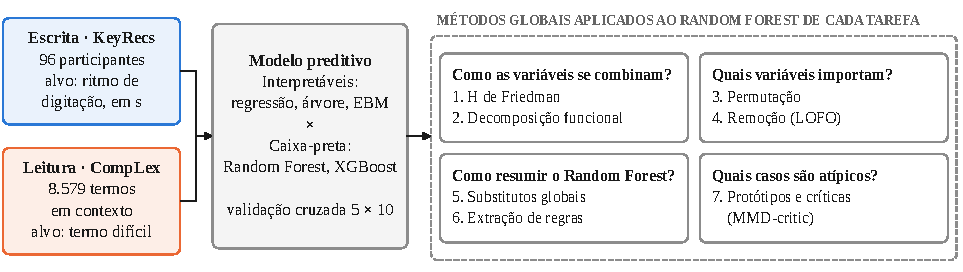
\includegraphics[width=\textwidth]{figuras/fluxo.pdf}
\caption{Fluxo da análise nas duas bases}
\label{fig:fluxo}
\fonte{elaborado pelos autores com a biblioteca Matplotlib, do Python.}
\end{figure}

\subsection{Escrita: base KeyRecs}

A KeyRecs \citep{dias2023} registra os tempos de cada tecla de participantes
que redigitaram uma senha fixa cerca de 100 vezes em cada uma de
duas sessões e depois transcreveram um texto. A limpeza descartou pausas acima de
10 s, repetições corrompidas e três participantes com ritmo mediano menor ou
igual a zero, típico de quem digita sobrepondo teclas; restaram 96
participantes, que formam a unidade de análise. A variável resposta é o ritmo de digitação na transcrição:
a mediana do tempo de voo (intervalo entre soltar uma tecla e apertar a
seguinte), em segundos. Por ser uma mediana, ela descreve o ritmo típico da
pessoa, e não as pausas longas, e serve de linha de base individual, acima da
qual uma pausa pode ser tratada como hesitação. Para verificar essa ligação, a
análise de importância foi repetida com a taxa de pausas longas como alvo, isto
é, a proporção de intervalos acima do percentil 90 de todos os intervalos do
texto. As sete variáveis explicativas são quatro medidas da senha (tempo de
voo, tempo de pressionamento da tecla, coeficiente de variação do tempo total
entre repetições e ganho com a prática da primeira para a segunda sessão) e
idade, gênero e lateralidade. Ao conferir a base, verificamos que os rótulos
das colunas de pares de teclas estão trocados no arquivo da senha; o tempo de
voo foi calculado com a pausa real.

\subsection{Leitura: base CompLex}

O CompLex \citep{shardlow2020} reúne termos em inglês, cada um na frase em que
aparece, retirados da Bíblia, de artigos biomédicos e de atas
do Parlamento Europeu e anotados por leitores quanto à complexidade. Usamos os
8.579 termos de uma palavra e consideramos difícil o termo com complexidade
média de pelo menos 0,5 (9,7\% dos casos), como aproximação do termo que o
leitor buscaria. As oito variáveis foram calculadas a partir do texto:
frequência no idioma, na escala Zipf, obtida da biblioteca wordfreq; comprimento; número de sílabas; sigla; nome próprio; tamanho
da frase; posição do termo na frase; e forma em português, igual a 1 quando a
mesma grafia também é frequente em português. A frequência tem correlação de
$-0,63$ com a complexidade.

\subsection{Modelos preditivos}

Para prever o ritmo de digitação, comparamos a previsão constante pela mediana, a
regressão linear, uma árvore de decisão podada e um Random Forest
\citep{breiman2001}, pelo RMSE em validação cruzada com 5 dobras repetida 10
vezes. Para classificar os termos, comparamos uma regra baseada só na
frequência, a regressão logística, uma árvore podada, o EBM
\citep{lou2013}, o Random Forest e o XGBoost. O EBM é
um modelo aditivo generalizado em que cada variável contribui por uma função de
forma que pode ser lida num gráfico. Como a mesma palavra aparece em várias
frases, as dobras foram agrupadas por palavra. As métricas foram a AUC e a
precisão nos 10\%, a proporção de termos difíceis entre os 10\% com maior
probabilidade prevista, que corresponde ao uso pretendido do assistente. Os
hiperparâmetros foram escolhidos em 70\% dos dados, e as diferenças entre
modelos foram testadas pelo teste $t$ corrigido para validação cruzada
\citep{nadeau2003}.

\subsection{Métodos de explicabilidade}

Os sete métodos globais foram aplicados ao Random Forest de cada tarefa. A estatística H de Friedman \citep{friedman2008} mede, de 0 a 1, a
fração da variação da previsão que se deve a interações; reportamos H, a raiz
de $H^2$. A decomposição funcional \citep{molnar2022} mede, pelo \Rdois, quanto
da previsão é reproduzido só pelos efeitos principais de cada variável. A
importância por permutação embaralha uma variável no modelo já treinado
\citep{breiman2001}, e a importância por remoção (LOFO) treina o modelo de novo
sem ela \citep{lei2018}; as duas foram calculadas nas mesmas 50 dobras, com o
teste $t$ corrigido e a correção de Holm para comparações
múltiplas. Uma árvore de profundidade 3 e uma regressão linear foram treinadas
para imitar o Random Forest, como modelos substitutos, e uma lista curta de
regras foi extraída das suas árvores \citep{friedman2008}; a fidelidade é o
\Rdois{} entre as previsões do resumo e as do Random Forest em 30\% dos dados
reservados para teste. Por fim, o MMD-critic \citep{kim2016} escolheu
protótipos, os casos que melhor representam os dados, e críticas, os casos
atípicos, com as variáveis padronizadas; na leitura, ele foi aplicado aos 832
termos difíceis.

% =====================================================================
\section{RESULTADOS E DISCUSSÃO}

\subsection{Desempenho dos modelos}

Nas duas tarefas, o modelo interpretável por construção alcançou a caixa-preta
(Tabelas~\ref{tab:escrita} e~\ref{tab:leitura}). Na escrita, a regressão linear
teve o menor erro, com RMSE de 0,0314 s e \Rdois{} de 0,42, e a diferença para
o Random Forest não foi significativa ($p = 0,33$). A árvore podada fez um único
corte, tempo de voo na senha acima de 0,138 s, e já explicou 30\% da variação.
Na leitura, o EBM igualou o Random Forest em AUC (0,919 nos dois; $p = 0,82$), e
a regressão logística ficou próxima (0,914; $p = 0,18$). A regra que usa só a
frequência já levou a AUC a 0,849. Nos melhores modelos, a precisão nos 10\%
ficou perto de 0,5: cerca de metade dos termos que o assistente sugeriria são
de fato difíceis, o que equivale a cinco vezes a proporção de difíceis na base.

\begin{table}[!htb]
\begin{minipage}[t]{0.48\textwidth}
\centering
\caption{Escrita (KeyRecs): desempenho em validação cruzada}
\label{tab:escrita}
\small
\setlength{\tabcolsep}{3pt}
\begin{tabular}{@{}lccc@{}}
\toprule
Modelo & RMSE (s) & MAE (s) & \Rdois \\
\midrule
Mediana & 0,0450 & 0,0360 & $-0,10$ \\
Regressão linear$^{\ast}$ & 0,0314 & 0,0250 & 0,42 \\
Árvore podada$^{\ast}$ & 0,0351 & 0,0284 & 0,30 \\
Random Forest & 0,0342 & 0,0274 & 0,34 \\
\bottomrule
\end{tabular}

\vspace{2pt}
{\footnotesize $^{\ast}$Interpretável por construção. Random Forest contra
regressão linear: $p = 0,33$.\par}

\fonte{elaborado pelos autores com a biblioteca pandas, do Python.}
\end{minipage}\hfill
\begin{minipage}[t]{0.48\textwidth}
\centering
\caption{Leitura (CompLex): desempenho em validação cruzada agrupada por palavra}
\label{tab:leitura}
\small
\setlength{\tabcolsep}{3pt}
\begin{tabular}{@{}lcc@{}}
\toprule
Modelo & AUC & Prec. 10\% \\
\midrule
Regra das palavras raras$^{\ast}$ & 0,849 & 0,382 \\
Regressão logística$^{\ast}$ & 0,914 & 0,506 \\
Árvore podada$^{\ast}$ & 0,902 & 0,446 \\
EBM$^{\ast}$ & 0,919 & 0,496 \\
Random Forest & 0,919 & 0,491 \\
XGBoost & 0,922 & 0,500 \\
\bottomrule
\end{tabular}

\vspace{2pt}
{\footnotesize $^{\ast}$Interpretável por construção. Prec. 10\%: precisão nos
10\%. AUC do Random Forest contra EBM: $p = 0,82$;
contra regressão logística: $p = 0,18$;
contra XGBoost: $p = 0,12$.\par}

\fonte{elaborado pelos autores com a biblioteca pandas, do Python.}
\end{minipage}
\end{table}

\subsection{Aditividade e importância das variáveis}

A decomposição funcional ajuda a entender esse empate
(Tabela~\ref{tab:sintese}). Os efeitos principais, sozinhos, reproduziram as
previsões do Random Forest com \Rdois{} de 0,97 na escrita e de 0,93 na
leitura, e a estatística H das variáveis principais ficou entre 0,16 e 0,26. Na
leitura, essa quase aditividade explica por que o EBM, também aditivo, alcança o
Random Forest. Na escrita, a explicação é outra, porque a regressão é linear, e
não apenas aditiva. O efeito principal do tempo de voo no Random Forest é um
degrau perto de 0,14 s, que uma reta não reproduz: a regressão linear treinada
para imitar o Random Forest teve fidelidade negativa ($R^2 = -0,38$). Esse
degrau, porém, não trouxe ganho preditivo, e a reta manteve o menor erro.

Pela importância por remoção, uma variável dominou cada tarefa. Sem o tempo de
voo, o RMSE do Random Forest subiu 10,4 ms, ou 30\% (Figura~\ref{fig:lofo}a) ($p = 0,004$ após a
correção de Holm), e ele ficou em primeiro lugar em todas as partições
testadas; nenhuma outra variável da escrita diferiu de zero. O tempo de voo
sozinho deu o mesmo erro do modelo completo (34,8 contra 34,6 ms). Na leitura,
sem a frequência, a AUC caiu 0,167; sigla e comprimento também pesaram, com
quedas abaixo de 0,01, ainda significativas após a correção. A frequência
sozinha, porém, não basta (AUC de 0,808) e só junto do comprimento se aproxima
do modelo completo (0,901). Com a taxa de pausas longas como alvo, retirar o
tempo de voo aumentou o erro em 17\% ($p < 0,001$), o que apoia o uso do ritmo
previsto como referência para identificar hesitações.

\begin{figure}[!htb]
\centering
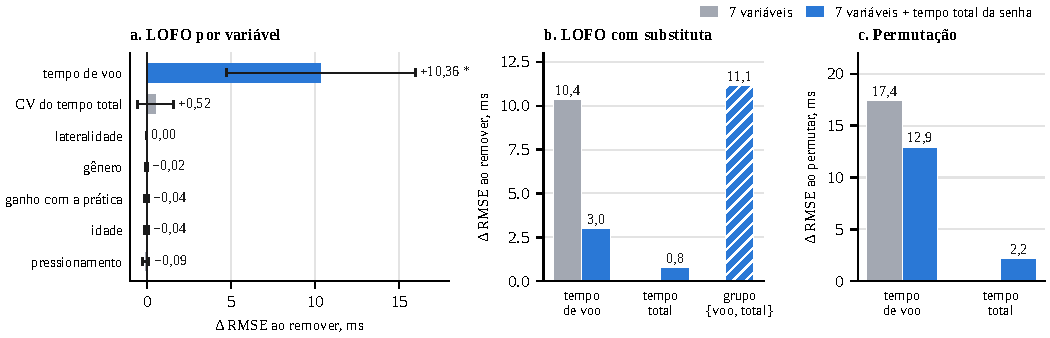
\includegraphics[width=\textwidth]{figuras/lofo_escrita.pdf}
\caption{Importância das variáveis na escrita: a) LOFO, com intervalo de 95\% (* $p < 0,05$); b) LOFO com o tempo total da senha no modelo; c) permutação nas mesmas dobras}
\label{fig:lofo}
\fonte{elaborado pelos autores com a biblioteca Matplotlib, do Python.}
\end{figure}

A comparação entre os dois tipos de importância mostrou quando eles divergem
(Figura~\ref{fig:lofo}b e~\ref{fig:lofo}c).
Ao devolver ao modelo o tempo total da senha, que tem correlação de 0,78 com o
tempo de voo, a importância por remoção do tempo de voo caiu 71\%, de 10,4 para
3,0 ms, e deixou de ser significativa, enquanto a importância por permutação
caiu 26\%, de 17,4 para 12,9 ms. Na leitura, comprimento e número de sílabas,
com correlação de 0,87, repetiram o padrão: removidos um de cada vez, pesam
pouco; removidos juntos, a perda aparece. A remoção mede a contribuição única
da variável, e a permutação mede quanto o modelo já treinado depende dela, mas
cria combinações de valores que não existem nos dados
\citep{hooker2021}. Os dois métodos respondem, portanto, a perguntas
diferentes. Por isso, convém relatá-los juntos e remover em grupo as variáveis
correlacionadas antes de concluir que alguma delas não importa.

\begin{table}[!htb]
\centering
\caption{Síntese dos sete métodos globais aplicados ao Random Forest}
\label{tab:sintese}
\small
\renewcommand{\arraystretch}{1.1}
\begin{tabular}{@{}>{\raggedright\arraybackslash}p{3.1cm}
                >{\raggedright\arraybackslash}p{5.9cm}
                >{\raggedright\arraybackslash}p{5.9cm}@{}}
\toprule
Método & Escrita (KeyRecs) & Leitura (CompLex) \\
\midrule
H de Friedman & Maior H: CV do tempo total e tempo de voo (0,17 e 0,16) & Maior H: frequência (0,26); par relevante mais forte: comprimento e sigla (0,27) \\
Decomposição funcional & Efeitos principais: \Rdois{} $= 0,97$ & Efeitos principais: \Rdois{} $= 0,93$ \\
Permutação & Só o tempo de voo difere de zero (17,4 ms) & Frequência (0,291 na AUC), comprimento e sigla (0,024 e 0,023) \\
Remoção (LOFO) & Só o tempo de voo: +10,4 ms, 30\% do RMSE & Frequência (0,167 na AUC), sigla e comprimento (0,009 e 0,008) \\
Substitutos globais & Árvore: \Rdois{} $= 0,98$; linear: \Rdois{} $= -0,38$ & Árvore: \Rdois{} $= 0,91$; linear: \Rdois{} $= 0,79$ \\
Extração de regras & 5 regras e SENÃO: \Rdois{} $= 0,90$ & 5 regras e SENÃO: \Rdois{} $= 0,79$ \\
Protótipos e críticas & Erro maior nas críticas: 0,043 contra 0,033 s & Críticas bem reconhecidas: probabilidade de 0,50 contra 0,41 \\
\bottomrule
\end{tabular}


\vspace{2pt}
\fonte{elaborado pelos autores com a biblioteca pandas, do Python.}
\end{table}

\subsection{Resumos legíveis e casos atípicos}

A árvore substituta e a lista de cinco regras reproduziram bem o Random Forest
(Tabela~\ref{tab:sintese}), e suas primeiras divisões repetem o que os modelos
interpretáveis já mostravam: tempo de voo acima de 0,138 s, na escrita,
e frequência abaixo de 3,38 na escala Zipf, seguida de comprimento e sigla, na
leitura. Essas fidelidades medem a semelhança com o Random Forest, e não com o
fenômeno estudado.

Os casos atípicos mostram onde cada modelo falha. Na escrita, entre as críticas
estão a participante com o maior tempo de voo na senha e o ritmo mais lento na
transcrição e um canhoto de 41 anos, perfis raros numa amostra com só 8
canhotos; o erro médio foi maior nas críticas (0,043 s) do que nos protótipos
(0,033 s). Na leitura, as críticas (três siglas, um nome próprio raro e uma
palavra muito longa) foram bem reconhecidas, com probabilidade média de 0,50,
contra 0,41 nos protótipos. As maiores falhas estão em outro lugar: palavras
comuns que os leitores acharam difíceis, como \emph{season} e \emph{matrix},
esta em \emph{mitochondrial matrix}, com probabilidade prevista abaixo de 0,01.
Nelas, a dificuldade vem do sentido técnico da palavra no contexto, que as
variáveis atuais não capturam.

\subsection{Alcance dos resultados}

Os resultados têm alguns limites. Na escrita, a amostra tem 96 participantes, e os métodos
avaliados num único conjunto de teste, como os substitutos e as regras, contam
com só 29 deles; com apenas 8 canhotos, também não é possível avaliar o efeito
da lateralidade. A tarefa é de transcrição, em que a pessoa copia um texto em
vez de compô-lo, e o alvo resume o ritmo típico de cada pessoa: o modelo não
prevê o momento de uma pausa, e pausas ligadas à escolha de palavras ou à
ortografia não foram medidas. Na leitura, o termo difícil é uma aproximação da
busca real, obtida por um corte em 0,5 numa escala contínua; os textos estão em
inglês, e a origem de cada texto não entrou como variável, embora casos como
\emph{matrix} sugiram que ela importa. Sigla, nome próprio e forma em português
foram definidos por regras simples sobre a grafia. Quanto aos métodos, a
estatística H é instável quando o efeito das variáveis é pequeno, H e as regras
podem mudar com outra partição dos dados, e no LOFO só o topo do ranking se
mostrou estável. Os hiperparâmetros foram escolhidos em 70\% dos dados, que
reaparecem como teste nas dobras, o que pode deixar o erro estimado um pouco
otimista; uma validação aninhada evitaria esse viés. Por fim, nenhuma dessas
medidas de importância é causal.

% =====================================================================
\section{CONCLUSÃO}

Nas duas tarefas, modelos interpretáveis por construção bastaram: a regressão
linear, na escrita, e o EBM, na leitura, alcançaram o Random Forest. Os métodos
globais mostraram que o Random Forest é quase aditivo, que uma variável
concentra o efeito em cada tarefa (o tempo de voo na senha e a frequência da
palavra) e que uma árvore pequena ou uma lista de cinco regras o resumem com
fidelidade de 0,79 a 0,98. Quando há variáveis correlacionadas, a importância
por remoção e a por permutação divergem, e relatar as duas evita concluir que
uma variável não importa.

Os resultados têm o alcance de uma amostra pequena na escrita, de um rótulo
aproximado na leitura e de modelos ainda não avaliados com usuários. Como
continuidade,
pretendemos modelar a hesitação no nível da palavra, usando o ritmo previsto
como referência, estender a análise da leitura ao português, incluir
representações do termo no contexto e avaliar o assistente com usuários.

% =====================================================================
% Referências conforme ABNT NBR 6023, em ordem alfabética e alinhadas à
% esquerda. O DOI é elemento complementar na NBR 6023 e foi omitido, como nos
% exemplos do modelo do evento. O texto entre colchetes define como cada obra aparece na citação.
\clearpage
\begin{thebibliography}{99}

\bibitem[Breiman(2001)]{breiman2001}
BREIMAN, L. Random forests. \textbf{Machine Learning}, v. 45, n. 1, p. 5-32,
2001.

\bibitem[Dias et al.(2023)]{dias2023}
DIAS, T.; VITORINO, J.; MAIA, E.; SOUSA, O.; PRAÇA, I. KeyRecs: a keystroke
dynamics and typing pattern recognition dataset. \textbf{Data in Brief}, v. 50,
109509, 2023.

\bibitem[Friedman; Popescu(2008)]{friedman2008}
FRIEDMAN, J. H.; POPESCU, B. E. Predictive learning via rule ensembles.
\textbf{The Annals of Applied Statistics}, v. 2, n. 3, p. 916-954, 2008.

\bibitem[Hooker; Mentch; Zhou(2021)]{hooker2021}
HOOKER, G.; MENTCH, L.; ZHOU, S. Unrestricted permutation forces extrapolation:
variable importance requires at least one more model, or there is no free
variable importance. \textbf{Statistics and Computing}, v. 31, n. 6, 82, 2021.

\bibitem[Kim; Khanna; Koyejo(2016)]{kim2016}
KIM, B.; KHANNA, R.; KOYEJO, O. O. Examples are not enough, learn to criticize!
Criticism for interpretability. In: CONFERENCE ON NEURAL INFORMATION PROCESSING
SYSTEMS, 30., 2016, Barcelona. \textbf{Advances in Neural Information
Processing Systems} [...]. Red Hook: Curran Associates, 2016. v. 29,
p. 2280-2288.

\bibitem[Lei et al.(2018)]{lei2018}
LEI, J.; G'SELL, M.; RINALDO, A.; TIBSHIRANI, R. J.; WASSERMAN, L.
Distribution-free predictive inference for regression. \textbf{Journal of the
American Statistical Association}, v. 113, n. 523, p. 1094-1111, 2018.

\bibitem[Leijten; Van Waes(2013)]{leijten2013}
LEIJTEN, M.; VAN WAES, L. Keystroke logging in writing research: using Inputlog
to analyze and visualize writing processes. \textbf{Written Communication},
v. 30, n. 3, p. 358-392, 2013.

\bibitem[Lou et al.(2013)]{lou2013}
LOU, Y.; CARUANA, R.; GEHRKE, J.; HOOKER, G. Accurate intelligible models with
pairwise interactions. In: ACM SIGKDD INTERNATIONAL CONFERENCE ON KNOWLEDGE
DISCOVERY AND DATA MINING, 19., 2013, Chicago. \textbf{Proceedings} [...]. New
York: ACM, 2013. p. 623-631.

\bibitem[Molnar(2022)]{molnar2022}
MOLNAR, C. \textbf{Interpretable machine learning}: a guide for making black
box models explainable. 2. ed. Munique: Christoph Molnar, 2022.

\bibitem[Nadeau; Bengio(2003)]{nadeau2003}
NADEAU, C.; BENGIO, Y. Inference for the generalization error. \textbf{Machine
Learning}, v. 52, n. 3, p. 239-281, 2003.

\bibitem[Rudin(2019)]{rudin2019}
RUDIN, C. Stop explaining black box machine learning models for high stakes
decisions and use interpretable models instead. \textbf{Nature Machine
Intelligence}, v. 1, n. 5, p. 206-215, 2019.

\bibitem[Shardlow; Cooper; Zampieri(2020)]{shardlow2020}
SHARDLOW, M.; COOPER, M.; ZAMPIERI, M. CompLex: a new corpus for lexical
complexity prediction from Likert scale data. In: WORKSHOP ON TOOLS AND
RESOURCES TO EMPOWER PEOPLE WITH READING DIFFICULTIES, 1., 2020, Marseille.
\textbf{Proceedings} [...]. Marseille: European Language Resources
Association, 2020. p. 57-62.

\end{thebibliography}

\end{document}
